\begin{frame}{Setup}
	\begin{itemize}
		\item Virtual world with a path
		\item Two groups
			\begin{itemize}
				\item Task
				\item Control
			\end{itemize}
		\item Walk through the physical room
		\item Adjust rotational gains
		\item Maintain presence
	\end{itemize}
	\note{
		So, let's get to the experiment that we designed.
		We're keeping as close as possible to the paper we're trying to reproduce of course, while staying within possible.
		
		There's two test group: One that just walks along the path normally, and one that gets some task while doing this, to see if that distracts them from noticing the gains.
		This task can be anything: We were initially thinking about having people count symbols on the walls or having a light that changes color.
		Ultimately, we settled on math problems.
		
		Presence is very important because people need to be really into the world.
		If we can keep the people present in the world, they will not notice it.
		Break the immersiveness.
	}
\end{frame}

\begin{frame}{Challenges}
	\begin{itemize}
		\item Positional tracking
			\begin{itemize}
				\item Bluetooth triangulating
				\item Oculus DK2 positional tracker
			\end{itemize}
		\item Broken Oculus
		\item 2 hours in the lab per week
	\end{itemize}
	\note{
		We've had some problems- ehrm, faced some challenges of course, during implementation.
		
		First off, positional tracking.
		Change world, need to know where they are.
		Bluetooth, Android, XY, slow.
		Luckily, lab DK2, pos tracker.
		Not really.
		Very small res.
		
		Add to that 2 hours blah.
	}
\end{frame}

\begin{frame}{Solutions}
	\only<1>{
		\begin{itemize}
			\item Gamepad \note{
				We gave up on doing real positional tracking, but we tried to keep it as real as possible by only allowing forward motion.
				This means that while people walked using the controller, they did have to rotate their bodies to change direcion.
			}
		\end{itemize}
	}
	\only<2>{
		\begin{columns}
			\column{0.38\linewidth}
				\centering
				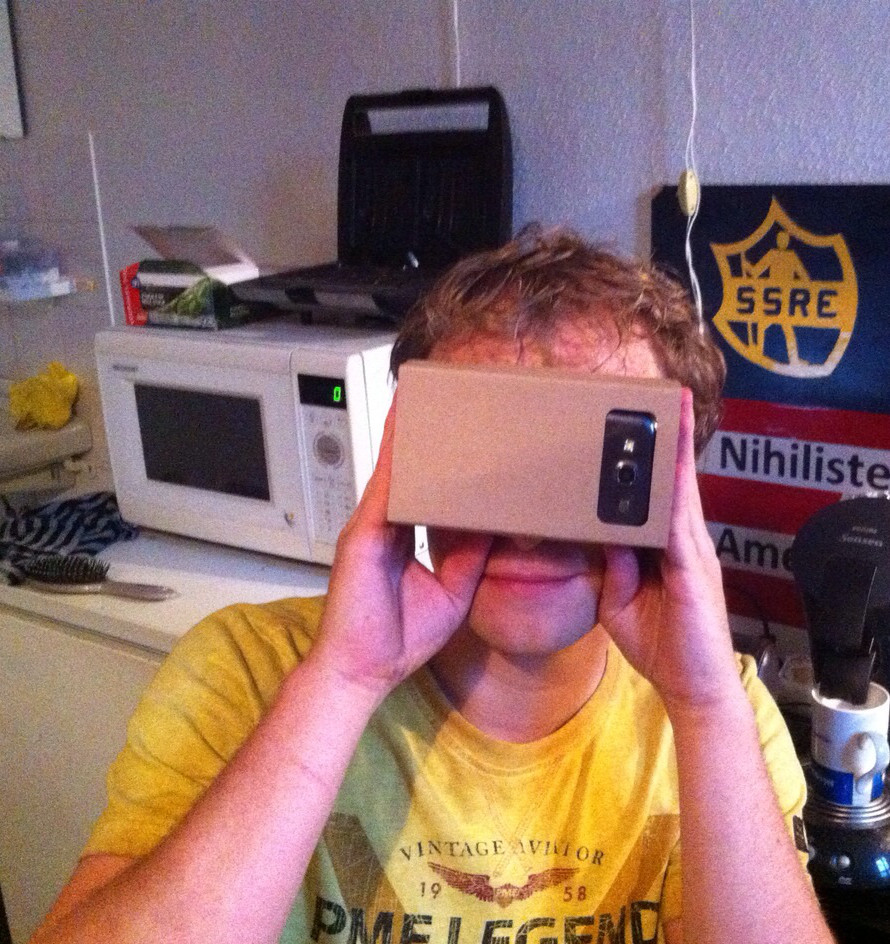
\includegraphics[width=\textwidth]{cardboard}
			\column{0.58\linewidth}
				\begin{itemize}
					\item Gamepad
					\item Google Cardboard (knock-off)
				\end{itemize}
		\end{columns}
	}
\end{frame}

\begin{frame}{Implementation}
	\begin{itemize}
		\item Oculus C++ SDK
		\item Rotational gains
			\begin{itemize}
				\item Change tracking code \note{This happens inside the SDK so not an option\\}
				\item Recalibrate Oculus \note{Not practical because you can't switch easily\\}
				\item Change FPS to influence rotation
				\item Interpret head rotation as extra mouse rotation \note{Weird jump between max and min value, this was noticable for negative gains\\}
			\end{itemize}
		\item Based on \emph{Tinyroom} SDK example
	\end{itemize}
\end{frame}


\begin{frame}{Implementation}
	\begin{figure}
		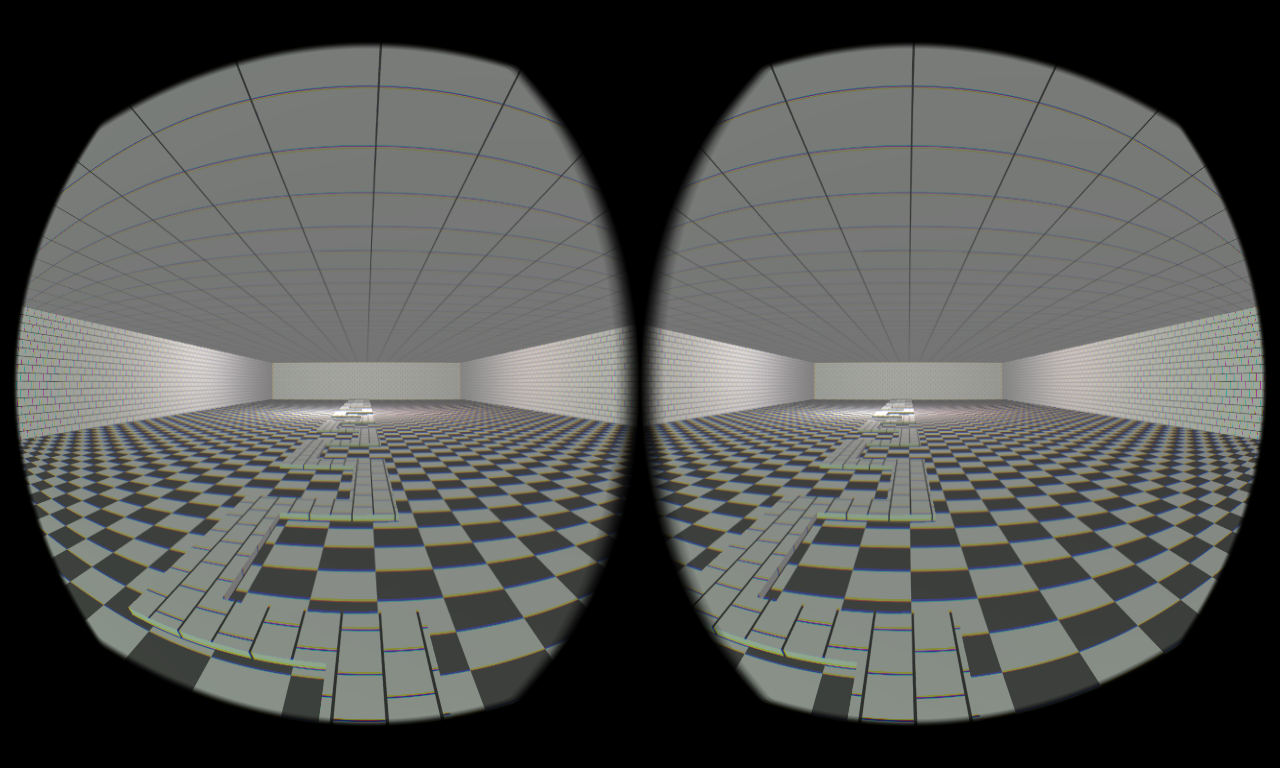
\includegraphics[height=0.8\textheight]{tinyroom}
	\end{figure}
\end{frame}

\begin{frame}{Execution}
	\begin{itemize}
		\item Metaforum
		\item Late at night \note{Because Fontys\\}
		\item Not hard to find subjects \note{Everyone was really excited\\}
		\item But, resetting and calibrating took a long time \note{Because of the jumps\\}
		\item 19 subjects
	\end{itemize}
\end{frame}

\begin{frame}{Execution}
	\begin{figure}
		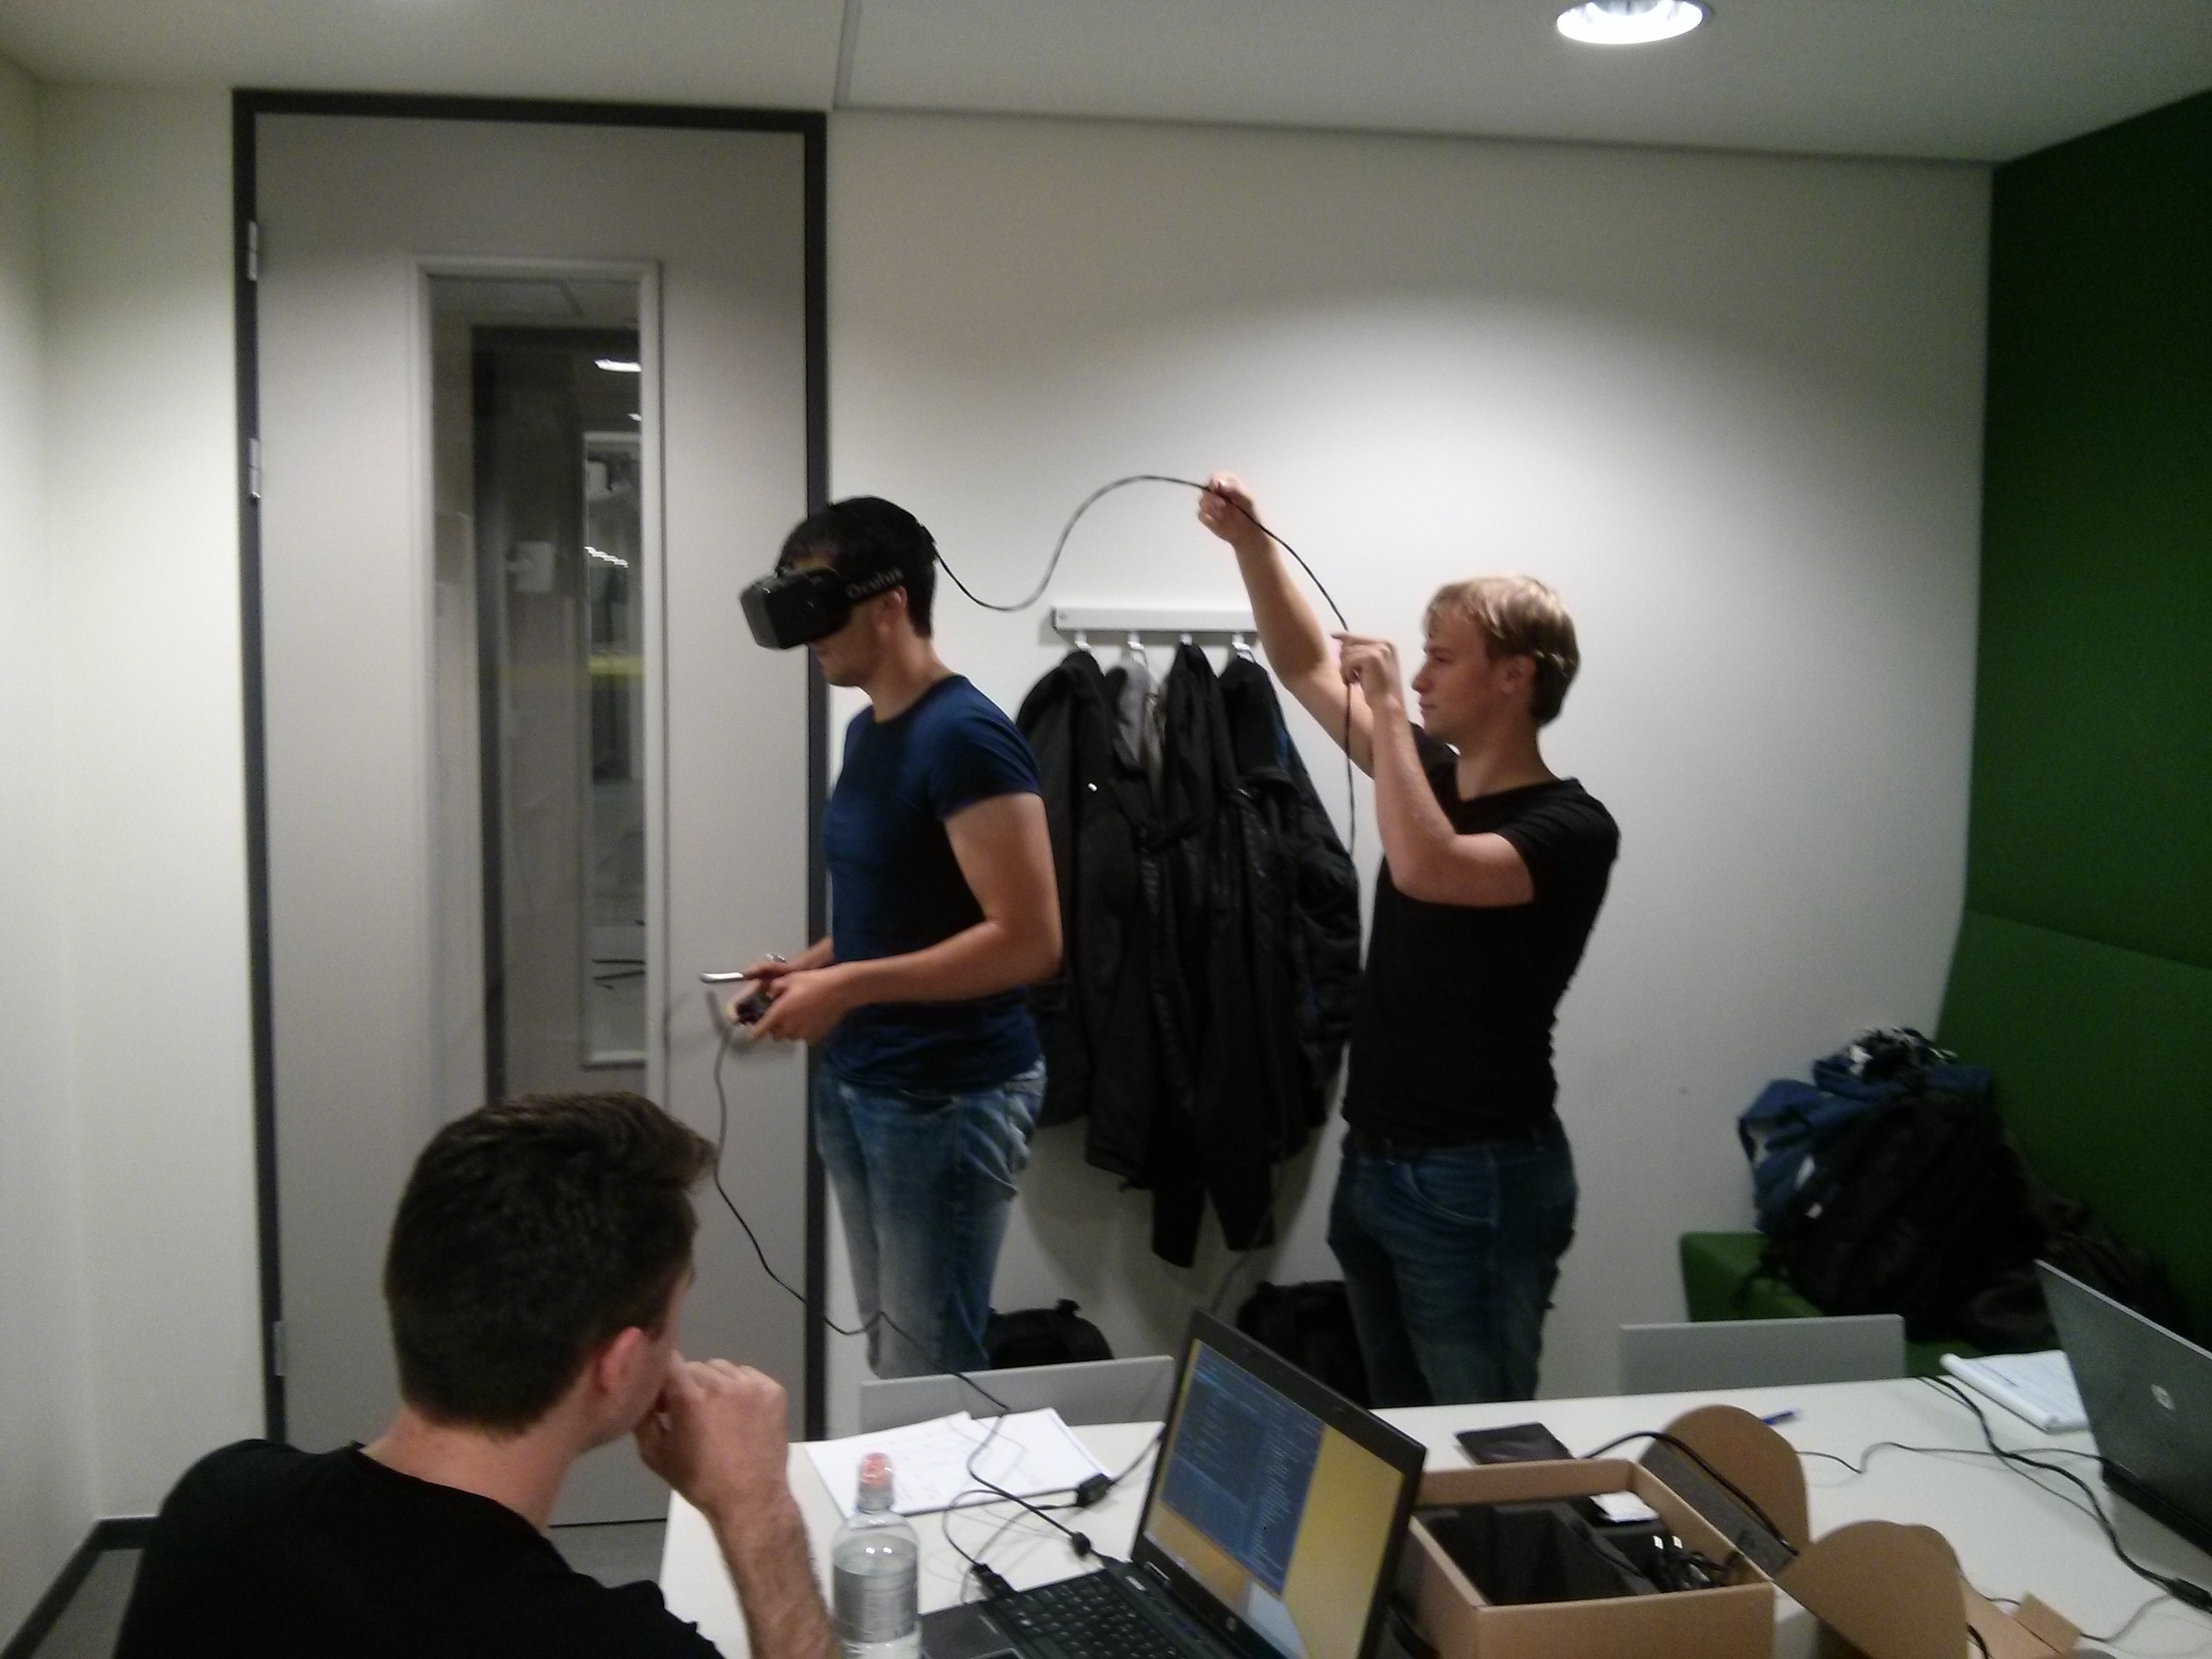
\includegraphics[height=0.8\textheight]{experiment}
	\end{figure}
	\note{Explain how we explained the experiment to the subjects, and what we asked:
		\begin{itemize}
			\item Gain
			\item Gender
			\item Calculation
			\item Notes on condition
		\end{itemize}
	}
\end{frame}
